\begin{problem}{51/figs/51_cubes.png}{Cubic Hole}  We are given a wooden cube with sides of length 1cm. We can drill the cube and create some holes of arbitrary shapes inside it. We then want to pass the largest possible cube thought the holes of the original cube. How would you drill the holes and what is the largest possible cube that can go through the holes?\\[0.2cm]
	
\textbf{More details:} 
The figure below shows an example of drilling the cube (The intersection of the cylinder and the cube is removed from the cube).
\begin{center}
	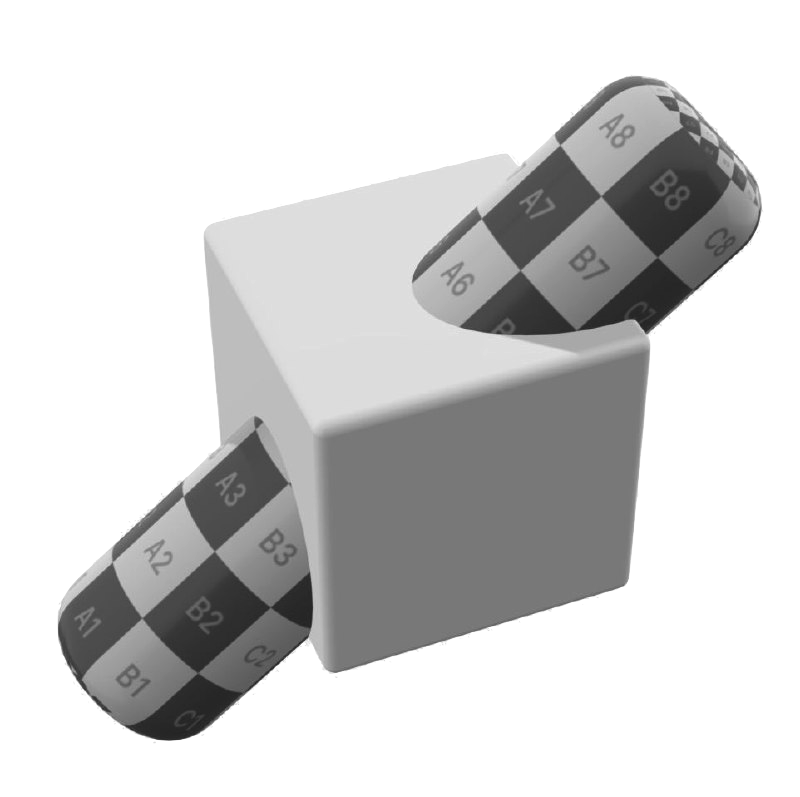
\includegraphics[width=5cm]{51/figs/51_1.png}
\end{center}
The cube should be drilled in a way that a thread can be passed through it and the cube can be hung by tying the two ends of the thread so that it cannot be pulled down without cutting the thread.

For example, in the figure below, you cannot hang the cube by tying the two ends of the thread.
\begin{center}
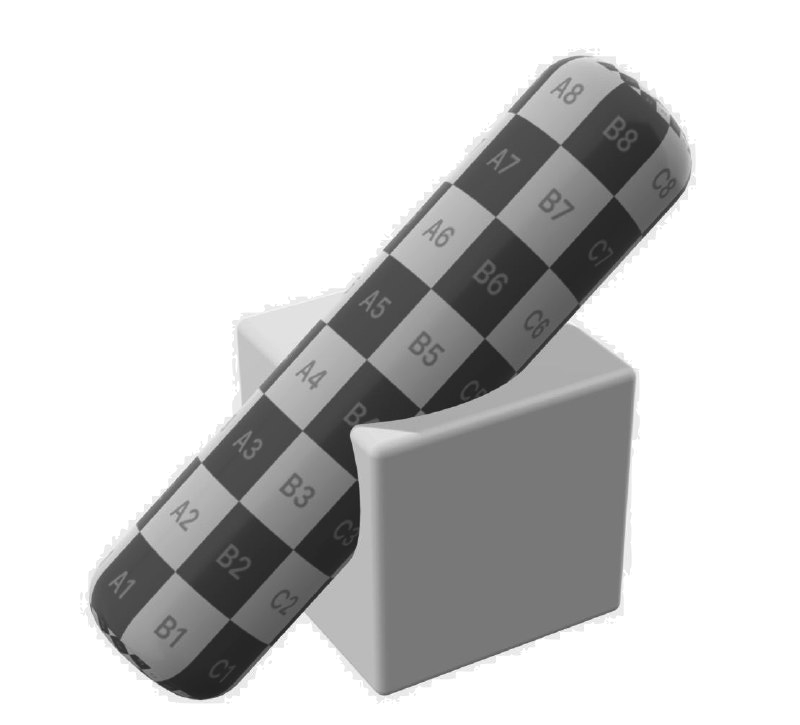
\includegraphics[width=5cm]{51/figs/51_2.png}
\end{center}

The passage of the second cube through the first cube should be such that the second cube can make a full circle around the hypothetical thread from which the first cube is hanging.
\end{problem}